\documentclass[a4paper, 11pt, onecolumn]{article} 

% arara: pdflatex 
% arara: bibtex
% arara: pdflatex
% arara: pdflatex
% arara: clean: {extensions: [ aux, bbl, out, toc, blg, thm ]}

\usepackage[doi, natbibapa]{apacite}

\usepackage{enumitem}
\usepackage[english]{babel}
%if french
%\frenchbsetup{StandardLists=true}

\usepackage[T1]{fontenc}
\usepackage[utf8]{inputenc}

\usepackage{lmodern}

\let\CheckCommand\providecommand
\usepackage{microtype}
\usepackage{hyperref}
%\usepackage[pagebackref=true]{hyperref}
%\renewcommand*{\backrefalt}[4]{#1}

\usepackage{lscape}
\usepackage{graphicx}
\usepackage{amssymb,amsmath}
\usepackage{url}
\usepackage{longtable}
\usepackage{tabu}
\usepackage{siunitx}                        
%\usepackage{threeparttable} 
\usepackage{array}
\usepackage{booktabs}

%\usepackage[french]{authblk}
%\DeclareCaptionFormat{twodot}{:}
\usepackage[font=small,skip=1em]{caption}


\usepackage{setspace}
\usepackage{fullpage}
\usepackage{eso-pic}

\usepackage[explicit, clearempty]{titlesec}
\usepackage[tableposition=top]{caption}
%\usepackage{titlesec}
\usepackage[a4paper]{geometry}

\usepackage{adjustbox}
\usepackage{rotating}
\usepackage{hvfloat}
\usepackage{wrapfig}
\usepackage{tfrupee}  
%\usepackage{multicol}

\usepackage{calc}

\usepackage{lettrine}
\usepackage{oldgerm}

\usepackage{fancyhdr}
\usepackage{lipsum}  
\usepackage{lastpage}

\usepackage{changepage}

% *****************************************************************
% Annexes
% *****************************************************************
%\usepackage[title, titletoc]{appendix}
\usepackage[toc,page]{appendix}
%\renewcommand\appendixtocname{Annexes}
%\renewcommand\appendixname{Annxes}
%\renewcommand\appendixpagename{Annexes}

% *****************************************************************
% Estout related things
% *****************************************************************
\newcommand{\sym}[1]{\rlap{#1}}

\let\estinput=\input% define a new input command so that we can still flatten the document

\newcommand{\estwide}[3]{
		\vspace{.75ex}{
			\begin{tabular*}
			{\textwidth}{@{\hskip\tabcolsep\extracolsep\fill}l*{#2}{#3}}
			\toprule
			\estinput{#1}
			\bottomrule
			\addlinespace[.75ex]
			\end{tabular*}
			}
		}	

\newcommand{\estauto}[3]{
		\vspace{.75ex}{
			\begin{tabular}{l*{#2}{#3}}
			\toprule
			\estinput{#1}
			\bottomrule
			\addlinespace[.75ex]
			\end{tabular}
			}
		}

% Allow line breaks with \\ in specialcells
	\newcommand{\specialcell}[2][c]{%
	\begin{tabular}[#1]{@{}c@{}}#2\end{tabular}}

% *****************************************************************
% Custom subcaptions
% *****************************************************************
% Note/Source/Text after Tables
\newcommand{\figtext}[1]{
	\vspace{-1.9ex}
	\captionsetup{justification=justified,font=footnotesize}
	\caption*{\hspace{6pt}\hangindent=1.5em #1}
	}
\newcommand{\fignote}[1]{\figtext{\emph{Note:~}~#1}}

\newcommand{\figsource}[1]{\figtext{\emph{Source:~}~#1}}

% Add significance note with \starnote
\newcommand{\starnote}{\figtext{* p < 0.1, ** p < 0.05, *** p < 0.01. Standard errors in parentheses.}}

% *****************************************************************
% siunitx
% *****************************************************************
\usepackage{siunitx} % centering in tables
	\sisetup{
		detect-mode,
		tight-spacing		= true,
		group-digits		= false ,
		input-signs		= ,
		input-symbols		= ( ) [ ] - + *,
		input-open-uncertainty	= ,
		input-close-uncertainty	= ,
		table-align-text-post	= false
        }

% *****************************************************************
% Sources
% *****************************************************************
\newcommand{\sourcetab}[1]{\vspace{-1em} \caption*{ \textbf{Source}: {#1}} }
\newcommand{\sourcefig}[1]{\vspace{-2em} \caption*{ \textbf{Source}: {#1}} }

\addto\captionsenglish{\renewcommand{\figurename}{\textbf{Figure}}}
\addto\captionsenglish{\renewcommand{\tablename}{\textbf{Table}}}


% *****************************************************************
% Abstract
% *****************************************************************
\let\abstractname\abstracteng

% *****************************************************************
% Hypothèses
% *****************************************************************
\usepackage{ntheorem}
\theoremseparator{:}
\newtheorem{hyp}{Hypothesis}

% \makeatletter
% \newcounter{subhyp} 
% \let\savedc@hyp\c@hyp
% \newenvironment{subhyp}
 % {%
  % \setcounter{subhyp}{0}%
  % \stepcounter{hyp}%
  % \edef\saved@hyp{\thehyp}% Save the current value of hyp
  % \let\c@hyp\c@subhyp     % Now hyp is subhyp
  % \renewcommand{\thehyp}{\saved@hyp\alph{hyp}}%
 % }
 % {}
% \newcommand{\normhyp}{%
  % \let\c@hyp\savedc@hyp % revert to the old one
  % \renewcommand\thehyp{\arabic{hyp}}%
% } 
% \makeatother

% *****************************************************************
% Tableaux
% *****************************************************************
\addto\captionsfrench{\def\tablename{\textsc{Table}}}

% *****************************************************************
% Bigcenter
% *****************************************************************
%%% ----------debut de bigcenter.sty--------------
 
%%% nouvel environnement bigcenter
%%% pour centrer sur toute la page (sans overfull)
 
%\newskip\@bigflushglue \@bigflushglue = -100pt plus 1fil
 
%\def\bigcenter{\trivlist \bigcentering\item\relax}
%\def\bigcentering{\let\\\@centercr\rightskip\@bigflushglue%
%\leftskip\@bigflushglue
%\parindent\z@\parfillskip\z@skip}
%\def\endbigcenter{\endtrivlist}
 
%%% ----------fin de bigcenter.sty--------------
%%%% fin macro %%%%
\makeatletter
\newskip\@bigflushglue \@bigflushglue = -100pt plus 1fil
\def\bigcenter{\trivlist \bigcentering\item\relax}
\def\bigcentering{\let\\\@centercr\rightskip\@bigflushglue%
\leftskip\@bigflushglue
\parindent\z@\parfillskip\z@skip}
\def\endbigcenter{\endtrivlist}
\makeatother

% *****************************************************************
% Lignes de code
% *****************************************************************
\usepackage{listings}
\lstset{ 
basicstyle=\scriptsize\ttfamily,
breaklines=true,
keywordstyle=\bf \color{blue},
commentstyle=\color[gray]{0.5},
stringstyle=\color{red},
showstringspaces=false,
numbers=left,
numberstyle=\tiny \bf \color{blue},
stepnumber=1,
numbersep=10pt,
firstnumber=1,
numberfirstline=true,
frame=leftline,
xleftmargin=0.5cm
}
 
% *****************************************************************
% Auteurs en bleu
% *****************************************************************
%\renewcommand{\citep}[1]{\textcolor{teal}{\citep{#1}}}
%\renewcommand{\cite}[1]{\textcolor{teal}{\cite{#1}}}
\usepackage{xcolor}
\usepackage{colortbl}

\hypersetup{colorlinks,linkcolor={red},citecolor={teal},urlcolor={blue}}
%\newcommand{\ypenser}[1]{\textcolor[purple]{#1}}
\newcommand{\ypenser}[1]{\textbf{\color{purple}--#1--}}

% *****************************************************************
% Mail
% *****************************************************************
\newcommand{\email}[1]{\href{mailto:#1}{\nolinkurl{#1}}}

% *****************************************************************
% Résumé et mots clés
% *****************************************************************
 \newenvironment{resab}[1]
{\begin{adjustwidth}{0cm}{0cm} \hangafter =1\par
    {\normalsize\bfseries #1\ \\ }\normalsize}
{\end{adjustwidth}\medskip}

 \newenvironment{keywords}
{\begin{adjustwidth}{0cm}{0cm} \hangafter =1\par
    {\normalsize\itshape Keywords:}~\normalsize}
{\end{adjustwidth}\medskip}

 \newenvironment{jelcodes}
{\begin{adjustwidth}{0cm}{0cm} \hangafter =1\par
    {\normalsize\itshape JEL Codes:}~\normalsize}
{\end{adjustwidth}\medskip}

% *****************************************************************
% Poete
% *****************************************************************
\newcommand{\attrib}[1]{%
\nopagebreak{\raggedleft\footnotesize #1\par}}

% *****************************************************************
% Stata
% *****************************************************************
\newcommand{\Stata}{%
\textsc{Stata$^{\mbox{\scriptsize{\textregistered}}}$}
}

% *****************************************************************
% Encadré
% *****************************************************************
\usepackage{tikz}

% Thick
\def\checkmark{\tikz\fill[scale=0.4](0,.35) -- (.25,0) -- (1,.7) -- (.25,.15) -- cycle;} 

\newcommand{\titlebox}[2]{%
\tikzstyle{titlebox}=[rectangle,inner sep=10pt,inner ysep=10pt,draw]%
\tikzstyle{title}=[fill=white]%
%
\bigskip\noindent\begin{tikzpicture}
\node[titlebox] (box){%
    \begin{minipage}{0.94\textwidth}
#2
    \end{minipage}
};
%\draw (box.north west)--(box.north east);
\node[title] at (box.north) {#1};
\end{tikzpicture}\bigskip%
}

% *****************************************************************
% Changer la forme des titres
% *****************************************************************
 %\titleformat{\section}[block]			%section + style prédéfini par l'extension (block = 1 ligne)
 %{\sffamily\bfseries\LARGE\titlerule[1pt]}						%format pour le titre + label
 %{\sffamily\bfseries\LARGE}						%format pour le titre + label
 %{\sffamily\bfseries\LARGE\arabic{section}}		%format que pour le label
 %{0.5cm}								%espace qui sépare le label du titre
 %{#1}									%description du style pour le titre uniquement
 %\titlespacing{\section}				%section
 %{0cm}									%espace à gauche du titre
 %{3em}									%espace verticale AVANT le titre
 %{1em}									%espace verticale APRES le titre
 %%{0cm} 								%espace à droite du titre: mettre la même valeur que gauche pour un peu centrer

 %\titleformat{\subsection}{\sffamily\bfseries\Large}{\thesubsection}{0.4cm}{#1}
 %\titlespacing{\subsection}
 %{1cm}
 %{2em}
 %{1ex}

 %\titleformat{\subsubsection}{\sffamily\bfseries\large}{\thesubsubsection}{0.4cm}{#1}
 %\titlespacing{\subsubsection}
 %{2cm}
 %{2em}
 %{1ex}

% *****************************************************************
% Style de la date
% *****************************************************************
%\def\mydate{\leavevmode\hbox{\the\year-\twodigits\month}}
\def\mydate{\leavevmode\hbox{\the\month-\twodigits\year}}
\def\twodigits#1{\ifnum#1<10 0\fi\the#1}

% *****************************************************************
% En tête
% *****************************************************************

% Pour les numéros de pages
%\pagestyle{fancy}

% Si tu veux mettre les numéros genre: 1/22
% Il faut que tu écrives
% "\thepage/\pageref{LastPage}"
% Sans les " " dans les lignes en bas: \fancyhead[...

% Ca c'est pour enlever la barre horizontale sous l'entête
% Pour la laisser tu mets "1pt" au lieu de 0
\renewcommand{\headrulewidth}{0pt}
\renewcommand{\footrulewidth}{0pt}

% fancyhead pour l'entête
% fancyfoot pour le pied de page
% L=left; R=right; C=center
%\fancyhead[L]{\textcolor{gray}{\textsf{\textit{Revue de la littérature autour du mariage: le cas de l'Inde}}}}
%\fancyhead[R]{\textcolor{gray}{\textsf{Natal, A. (\mydate)}}}
%\fancyfoot[C]{\thepage}
%updmap.exe --admin

%\lhead{\textcolor{gray}{\textsf{\textit{Revue de la littérature autour du mariage: le cas de l'Inde}}}}
%\rhead{\textcolor{gray}{\textsf{Natal, A. (\mydate)}}}
\cfoot{\thepage}

% *****************************************************************
% Jatis
% *****************************************************************
\newcommand{\jati}[1]{\textit{j\={a}ti{#1}}}

% *****************************************************************
% Enlever le titre Table des matières
% *****************************************************************
%\makeatletter
%\renewcommand\tableofcontents{%
%    \@starttoc{toc}%
%}
%\makeatother

% *****************************************************************
% À développer
% *****************************************************************
\newcommand\dev[1]{\textbf{\textcolor{red}{#1}}}

% *****************************************************************
% Fonts
% *****************************************************************
%\usepackage{tgbonum}
\usepackage{kpfonts}

% *****************************************************************
% Taille des tableaux
% *****************************************************************
\let\oldtabular=\tabular
\def\tabular{\small\oldtabular}
%\def\tabular{\normalsize\oldtabular}

% *****************************************************************
% Style de la biblio
% *****************************************************************
\bibliographystyle{apacite}

% *****************************************************************
% Numérotation
% *****************************************************************
%\usepackage{lineno}

% *****************************************************************
% Titre et page de garde
% *****************************************************************
\usepackage{titling}
\setlength{\droptitle}{-2cm}
\pretitle{\begin{center}\fontsize{24pt}{10pt}\selectfont\bfseries}
\posttitle{\par\end{center}\vskip 1ex}
\preauthor{\begin{center}
    \large \lineskip 0.5em}
\postauthor{\par\end{center}}
%\thanksheadextra{1,}{}
\thanksheadextra{}{}
\setlength\thanksmarkwidth{.5em}
\setlength\thanksmargin{-\thanksmarkwidth}


% *****************************************************************
% Symboles
% *****************************************************************

\def\@fnsymbol#1{\ensuremath{\ifcase#1\or *\or \dagger\or \ddagger\or
   \mathsection\or \mathparagraph\or \|\or **\or \dagger\dagger
   \or \ddagger\ddagger \else\@ctrerr\fi}}
   
\makeatletter
\newcommand{\ssymbol}[1]{^{\@fnsymbol{#1}}}
\makeatother
   
   
   
% *****************************************************************
% Makecell
% *****************************************************************
\usepackage{makecell}
\newcommand\Tablenote[2]{\multicolumn{#1}{l}{\makecell[l]{\textit{Note:}~#2}}}


   

%\usepackage{fonttable}

\usepackage{import}

\usepackage[
singlelinecheck=false % <-- important
]{caption}

\usepackage{upgreek}



% \renewcommand*\thetable{\Alph{section}.\arabic{table}}
% \renewcommand*\thefigure{\Alph{section}.\arabic{figure}}


% *****************************************************************
% Interlignes et marges
% *****************************************************************
\setstretch{1}
\geometry{%
left=2.5cm,
right=2.5cm,
top=2.5cm,
bottom=2.5cm,
%includefoot,
%headsep=1cm,
%footskip=1cm
}%




% *****************************************************************
% Page de garde
% *****************************************************************
%\title{Surviving debt, survival debt in times of lockdown\footnote{We sincerely thank Barbara Harriss-White, Judith Heyer and Jean-Michel Servet for their very helpful comments on an earlier draft.}}
\title{Surviving Debt, Survival Debt in Times of Lockdown\thanks{We sincerely thank Barbara Harriss-White, Judith Heyer and Jean-Michel Servet for their very helpful comments on an earlier draft.}}

\author{Isabelle Guérin\thanks{French National Research Institute for Sustainable Development (IRD), CESSMA (Université Paris Diderot, INALCO, IRD), French Institute of Pondicherry (IFP) - \email{isabelle.guerin@ird.fr}.}, ~Sébastien Michiels\thanks{CNRS-CREST, French Institute of Pondicherry (IFP).}, ~Arnaud Natal\thanks{Univ. Bordeaux, CNRS, GREThA, UMR 5113, F-33600 Pessac, France -- \email{arnaud.natal@u-bordeaux.fr}.}, ~Christophe J. Nordman\thanks{French National Research Institute for Sustainable Development (IRD), LEDa-DIAL (Université Paris-Dauphine, IRD, CNRS, PSL), French Institute of Pondicherry (IFP) - \email{nordman@dial.prd}.} ~and Govindan Venkatasubramanian\thanks{French Institute of Pondicherry (IFP).}}


\date{\today}



% ******************************************************************
\begin{document}

\maketitle

\hrule 
\vspace{0.3cm}

\begin{resab}{Abstract}
This article focuses on the consequences of the Indian lockdown in terms of debt. It is based on an ongoing study in a rural area of Tamil Nadu, South India. It draws on a long-term knowledge of this region, longitudinal quantitative household survey data on employment, debt and assets (2010-2016/17) as well as qualitative surveys conducted by telephone since the beginning of the lockdown in March 2020. 
Our results show: (i) the drying up of part of farm income and the bulk of off-farm income; (ii) the limited role of cash saving and cash transfers; (iii) the debt burden, since the population has faced massive debt growth over the past decade and some households are already very financially fragile; (iv) a predominance of informal finance with, however, a rise in finance; (v) a suspension of repayments, including for most informal lenders; (vi) a halt to unsecured debt and an erosion of the trust that cements most transactions; (vii) finally, the emergence of new forms of secured debt that threaten household assets. The sharp rise in debt observed over the last decade is the result of a widening of credit opportunities, partly formal but mostly informal. These have been made possible by building new relationships of trust but also of confidence in the future, based on strong economic growth that was believed to be sustainable. The lockdown highlights the fragility of these dynamics. For the poorest (mostly, but not only, Dalits), neither the state nor intra-caste or kinship solidarity are sufficient as a safety net. Impoverishment and a return to old forms of dependency seem to be the only way out.  

\end{resab}

\begin{motkey}{Keywords}
Debt, lockdown, caste, employment, India, Trust.
\end{motkey}


\hrule
%\linenumbers



% ******************************




\section*{Introduction}
\label{section:introduction}
What does ``lockdown'' mean in a context in which people depend on mobility and debt to make a living? In economies like India in which informal and vulnerable employment is the rule rather than the exception, and in which social protection remains the privilege of a minority, debt and movement are necessary for survival and protection. 
While much attention has been paid to informal labour and migration, this article focuses on the consequences of the lockdown in terms of private debt. It is based on an ongoing study in a rural area of Tamil Nadu, South India.

Researchers, activists and journalists have already warned of the dramatic consequences of the lockdown in the Global South. 
Martin Ravallion, for instance, anticipates that the response to the pandemic could turn into famine. 
He underlines the trade-off between two components of health: “illness due to the virus, and hunger and poor nutrition resulting from economic isolation and disruption to markets and institutions, including private social protection” \citep{Ravallion2020}\footnote{The World Food Programme plans that acute hunger could double by the end of 2020 and that 130 million lives and livelihoods will be at risk.}. 
The issue is of particular concern in India.
Strong lockdown measures were taken as early as March 24, first for three weeks and then extended until 31st of May (at the time of the writing). 
Soon after the lockdown, Jayati Ghosh, economist at Jawaharlal Nehru University, considered that “it has already completely destroyed the urban economy”, and it is a “much bigger stroke than the demonetization” \citep{Thapar2020}. Since then, various investigations have been carried out by researchers, activists and journalists to better appreciate the magnitude of the consequences. This body of research and reflection confirms the dramatic consequences of the lockdown, described as ``the greatest human tragedy in India's recent history'' \citep{Bhagat2020}, that could take us back to a time of a “Republic of Hunger” \citep{Deshpande2020}. After the demonetization (November 2016), the Goods and Services Tax reform (July 2017), the lockdown, quickly coupled with the dismantling of several labour laws\footnote{In mid-May, the states of Uttar Pradesh and Madhya Pradesh have introduced drastic proposals to deregulate labour laws in order to boost economic recovery after the lockdown: see \url{https://thewire.in/labour/labour-law-reform-worker-protection} (accessed on 29.05.20).},  can be considered as “a declaration of war on casual or bonded migrant labour” \citep{Harriss-White2020}.

The consequences of the lockdown on informal labour, both present and future, rightly give rise to a great deal of concern \citep{ILO2020, Majid2020}. This is particularly the case in India, where informal employment is estimated at 80-90 percent of the labour force \citep{ILO2016, Harriss-White2020, Srivastava2020}. The vast majority of these informal workers therefore no longer have any source of income. The most vulnerable are internal migrants, who account for a considerable share of employment. According to the most recent estimate, the number of vulnerable migrant workers ranges from 115 to 140 million \citep{Srivastava2020}. When the lockdown was announced, some of them returned home, often in dramatic conditions, either in crowded buses, on foot due to lack of transport \citep{Bhagat2020, Mukho2020, Picherit2020}. Others were trapped on the spot, left behind in miserable conditions \citep{Sahas2020}\footnote{A study carried out immediately after the lockdown among about 3,200 construction workers (the largest employment sector, with about 55 million workers all over India) displays a “dismal” picture of negligence and apathy (\cite{Sahas2020}, i): 42 percent of the workers mentioned that they had no ration left even for the day, 66 percent considered they will not be able to manage beyond a week and 22 percent of households mentioned they could manage for a month. 33 percent were still stuck in destination cities with little or no access to food, water and money. See also \cite{Bercegol2020}.}.  

While the issue of employment and labour is of course crucial, another aspect is also critical: that of private debt. Private debt, in India and elsewhere, has increased massively in recent decades.  According to UNCTAD analyses, based on MFI data, the global stock of debt, compared to GDP, has returned to its pre-global financial crisis level (260 percent in 2017, as opposed to 240 percent at the onset of the global financial crisis and 140 percent in 1980). This growth has largely been driven by the rise in private debt, which has increased more than 12-fold since 1980 and accounted for two-thirds of global debt in 2017. Developing countries, where private debt has long been confined to relatively low levels, are following the same trend: as a share of global GDP, private debt rose from 79 percent in 2008 to 139 percent in 2017 and is largely driven by non-financial corporations. ``The unprecedented explosion of private debt should clearly raise the loudest alarm bells'' (\cite{UNCTAD2019}, 74–75), all the more that a large part of this debt finances social reproduction rather than investment (ibid, 83). The latest World Bank report also warns of the crisis risks of a new wave of debt, both public and private, in developing countries \citep{WorldBank2020}. A UN report denounces the human rights deprivations linked to unsustainable levels of private debt \citep{UN2020}. The available data sometimes considerably underestimate actual indebtedness, as they do not, or poorly take informal indebtedness into account, which remains high in many contexts \citep{Collins2009, Demirguc2018}. Again, this is particularly the case in India  \citep{Gregory1997, Nair2016}. In our survey area, the NEEMSIS, informal debt represents 70 percent of household outstanding debt in volume.

This rise in private debt, in India and other parts of the Global South, is the outcome of several factors \citep{Servet2013, UN2020}. Low and irregular real incomes are one such factor, given the persistence of informal and vulnerable employment \citep{ILO2018}. Expenses are meanwhile increasing. Self-consumption, long a pillar of food security for rural families, has declined sharply over the last decades. Access to basic services such as water, electricity, housing and healthcare are becoming increasingly commodified. There has been an explosion of private provision of education, including among poor households seeking a better future for their children. The depletion of certain natural resources and of hitherto free common goods (drying up of groundwater, the disappearance of forest areas or restricted access to them, etc.) is causing substantial loss of earnings for some segments of the population. The adoption of urban lifestyles has led to a considerable increase in the supply of new goods, both identity and functional in nature. This is the case of mobile phones, but also household appliances, computers, internet access, motor vehicles (motorcycles or cars). 

The combination of strong economic growth and growing inequality \citep{Chancel2019}, typical of the Indian economy but also of many emerging countries, is fueling strong aspirations for social mobility. These can translate into the acquisition of sustainable consumer goods, a sign of integration into the consumer society \citep{Saiag2020, Gonzalez2015}. Aspirations can also translate into social investments such as marriage alliances, as in South Africa or India \citep{James2015, Srinivasan2005}. In the face of uncertain labour markets, matrimonial alliances can be a perfectly rational strategy for social mobility, or simply for security, especially for women \citep{DeNeve2016}. In addition to this, access to credit (the flip side of debt) can be in itself experienced as a source of recognition and emancipation, compared to other sources of debt that are considered oppressive because they are embedded in unequal social relations such as class, race, caste, kinship or gender. This is the case, for example, for working classes in Argentina \citep{Saiag2020} or Chile \citep{Gonzalez2015}. 
This is also observed in South Africa for the black community \citep{James2015}. It is the case in India for the Dalits, as we shall see here.

For households that are already massively indebted, and at a time when their sources of income are seriously affected, what will be the consequences of the lockdown? In some countries, regulatory moratoriums force credit providers to suspend repayments. This is observed in India and this is obviously very good news for borrowers, at least in the short term. But what about informal lenders, who still represent the bulk of debt sources? And in order to survive the day-to-day, do households have the possibility of taking on new debts to cope with their falling income? In the absence of income, won't they be forced to mortgage assets and what will be the consequences? The drop in income is obviously dramatic in the short term. The loss of assets is even more dramatic because it threatens future security, and the scale of a crisis can be measured precisely by the size of the assets destroyed \citep{Rhyne2020}. In addition to physical capital (land, housing, agricultural equipment, gold), reputation and trust play a crucial role since both largely condition creditworthiness (and access to employment). The embeddedness of economic transactions in personal relationships, typical of informal economies \citep{Platteau1994, Hart2000}, remains a predominant reality in India \citep{Harriss-White2003}.

This article is an attempt to answer these questions. It draws on a long-term knowledge of a region of Tamil Nadu, longitudinal data on employment, debt and assets (2010-2016/17) as well as qualitative surveys conducted by telephone since the beginning of the lockdown (\ref{section:data}). Our results can be summarized as follows: the drying up of part of farm income and the bulk of off-farm income (\ref{section:income}); the limited role of cash saving and cash transfers (\ref{section:saving}); the debt burden, since the population has faced massive debt growth over the past decade and some households are already very financially fragile (\ref{section:burden}); a predominance of informal finance with, however, a rise in formal finance (\ref{section:finlandscape}) a suspension of repayments, including for most informal lenders (\ref{section:repayment}); this goes along with a halt to unsecured debt and an erosion of the trust that cements most transactions (\ref{section:trust}); and finally the emergence of new forms of secured debt (some of which are old forms that had disappeared) that threaten household assets (\ref{section:newforms}).

The conclusion will discuss the implications and lessons of our findings. We will also briefly discuss the gendered effects of our results, although these would deserve further analysis. Far beyond being only a financial transaction, debt (and its flip side, credit), is a social relationship, which can be one of mutual aid and solidarity as well as one of power and hierarchy \citep{Mauss1993, Peebles2010}. The financial landscape of the region under study has been profoundly transformed in recent decades, and these transformations are inseparable from deep agrarian, economic and social transformations: the decline of agriculture, access to non-agricultural employment outside the village, a relative emancipation of Dalits from upper castes, both in terms of labour and debt, and a strengthening of Dalit solidarity, including regarding access to debt. The sharp rise in debt is the result of a widening of credit opportunities, partly formal but mostly informal. These have been made possible by building new relationships of trust but also of confidence in the future, based on strong economic growth that was believed to be sustainable. The lockdown highlights the fragility of these dynamics. For the poorest (mostly, but not only, Dalits), neither the state nor intra-caste or kinship solidarity are sufficient as a safety net. Impoverishment and a return to old forms of dependency seem to be the only way out.



\section{Data and context}
\label{section:data}


Our findings rely on an original socio-economic survey conducted in rural Tamil Nadu and combines quantitative and qualitative data. 
Quantitative data include the NEEMSIS household and individual survey, conducted in 2016-17 and which focused on all aspects of rural life, including in-depth questionnaire modules on labour arrangements (including migration), financial practices (debt and saving), consumption, remittances, access to governmental schemes, etc\footnote{The Networks, Employment, dEbt, Mobilities and Skills in India Survey (NEEMSIS) has been implemented in 2016-2017 by the authors of this paper. NEEMSIS follows a first household survey wave conducted in 2010 (RUME), thus constituting a panel of households and individuals. The first wave (RUME) was conducted among 405 households spread out in ten villages located in coastal/central Tamil Nadu in the Cuddalore and Villupuram districts. The villages were first selected following agro-ecological considerations (dry and wet villages) and the household sampling frame was made randomly using a caste stratification of the village populations obtained from the village Panchayats. For further details, see the survey dedicated website \url{https://neemsis.hypotheses.org/} and the NEEMSIS survey manual and statistical report \citep{Nordman2017, Nordman2019}.}. In total 2,692 individuals from 492 households were surveyed, spread across 19 villages in rural Tamil Nadu in the Cuddalore, Villuppuram, Kancheepuram, and Tiruppur districts. The original households and villages were randomly selected in 2010, using a stratified sample based on caste and location in terms of agricultural intensity and distance to town, and constituted then the sampling frame for collecting a panel dataset\footnote{To compare monetary values accross time, we deflate the values of 2016 on the basis of Consumer Price Index of World Bank in order to obtain values in base 2010 (\url{https://data.worldbank.org/indicator/FP.CPI.TOTL?locations=IN}).} in 2016-17. 
The data collection took place during harvest season. 
Incidentally, a break in the survey in 2016-17 occurred, partly due to the demonetization shock in November 2016. 
We took this opportunity to use the survey as a quasi-experimental design, allowing us to compare the situations of households before and after demonetization \citep{Guerin2017, Hilger2020}. 
Our results showed that demonetization had strong effects on employment, daily financial practices, and social network use for more than three months, as people relied more heavily on their networks to sustain their economic and social activities \citep{Guerin2017}. 
In addition, we found that this common shock had differential effects on levels of interpersonal trust, given the type of interactions that took place as a result of the shock. 
Notably, we highlighted an homophily principle in network use, where interactions that happened within a homogeneous group (neighborhoods for lower castes, kin and other caste members for upper castes) fostered trust, while outside interactions or relying on marginal ties decreased it \citep{Hilger2020}. 
While one of the main objectives of demonetization was the fight against corruption and the illegal economy, we rather observed that the shock had mostly strengthened the informal economy, and marginalised further those who lack effective support networks within their own community (caste group). 
As we will see in this paper, the lockdown effects are totally different: not only many economic transactions are reduced and even blocked, but also, pre-existing informal social interactions are discouraged and prohibited. 
Above all, uncertainty on the future is so high that it prevents both forms of exchanges. 
At the same time, new forms of financial transactions, based on physical collateral, are emerging.

The NEEMSIS data took place in a broader and still ongoing research programme launched in 2003, centred around questions on labour and finance behaviour and situated in coastal/central Tamil Nadu (South India).
In addition to quantitative surveys, various qualitative tools have been used since 2003. 
Concerning finance, the objective was to better capture the social and moral significance of financial practices, the way they interrelate with various social institutions such as caste, gender, class and the role that finance plays in the dynamics of social mobility and daily survival. 
Qualitative tools include life histories, which reconstruct family trajectories over time and the role of finance in the different stages of the life cycle; financial diaries, which trace all the financial flows of a residential unit; observation, which capture the nature of the relationship between lender and creditor and the modes of enforcement; informal interviews, which capture the lived experience of financial practices and the reasons why people, when given the choice, prefer this or that instrument. 

This long-term presence in the same field has enabled us to build special relationships with villagers, from landowners and local politicians to daily labourers, both men and women. 
At the time the lockdown was announced, many villagers contacted us by phone to obtain information about the duration of the lockdown, government programmes, sales opportunities for farmers' products, etc.
We took advantage of these spontaneous requests to ask them about their perception and their copying mechanisms. 
We also helped set up a food distribution system, a measure that we felt was ethically indispensable given our long-term commitment to the region. 
Our qualitative analysis combines our previous knowledge of the region with these telephone interviews. 

The original studied zone is economically dynamic, featuring a large proportion of irrigated agriculture, two industrial towns (Neyveli and Cuddalore) and a regional business centre (Panruti). 
Vanniyars and Paraiyars are the two major local groups across the region. 
Vanniyars can be qualified as “middle castes”. 
They are a farming caste with a low ritual rank, but in the villages we studied, as in many places in northeast Tamil Nadu, they control much of the land and are politically dominant\footnote{There are also a few Padayachis, Gramanis, Navithars, Nattars, Kulalars and Asarai, who have a similar position in the caste hierarchy.}. 
Paraiyars are one of the major Dalit communities in Tamil Nadu. 
There are also few Arunthathiyars among the Dalits in the studied zone. 
The upper castes of the local hierarchy are the Mudaliyars, Chettiyars, Naidus, Reddiyars, Settus and Yathavars, who account for only a small proportion of the village population. 
Christians and Muslims are a minority in the area. 
Lower castes or Dalits represent 46.5 percent, middle castes 44 percent and upper castes 9.5 percent of the NEEMSIS sample.

The region has seen many changes over the last three decades. 
Upper castes have mostly moved away from the villages to nearby towns, adopting urban jobs and lifestyles, and selling an important part of their land to Vanniyars. 
Overall, upper castes still have a hold on village life but are not as powerful as they used to be \citep{Harriss2013}. 
Land transfers to Vanniyars explain in great part why they are now dominant \citep{Harriss2016}, given that their dominance is permanently contested, including by Dalits \citep{Pandian2000}. 
As for Dalits, although their situation has been improving thanks to the combination of short term migration to nearby towns and industrial centres, and governmental schemes (reflected by subsidized housing, food, education, etc.; \citeauthor{Guerin2014}, \citeyear{Guerin2014})\footnote{For converging findings on other parts of Tamil Nadu, see \cite{Heyer2012, Harriss2016}}, inequalities persist.
In terms of education (Table \ref{Global}), looking at household heads, 58 percent of Dalits had not completed primary education level in 2016-17, compared to 38 percent of middle caste and 23 percent of upper caste household heads. 
Looking at incomes, the average annual income of Dalit households is INR 112k (median 68k), compared to INR 118k for middle and upper castes (median 82k and 103k respectively).
In terms of assets (land and house value, gold owned, value of livestock and farm equipment and value of consumer durable), Dalit households exhibited in 2016-17 an average value of INR 352k, while middle castes and upper castes households held respectively INR 1,098k and INR 1,263k.
The important decrease in asset values (38 percent) for upper caste households between 2010 and 2016-17 may be explained by the process of land transfer to middle castes households between the two years (see Table \ref{Global}).
It is likely that for some of them, the sale of land has allowed for urban investments (such as loans or transport), which the survey does not capture. 
For Dalits and middle-caste, the loss of land is probably the result of a non-choice: a sale to pay off a debt or to pay for a marriage.

Before exploring debt issues, let us take a quick look at the structure of employment and the impact of the lockdown on employment earnings.



\section{The drop in income: real but unequal}
\label{section:income}

What happened to labour and income under the lockdown? Like elsewhere in India, non-farm income is now largely dominant across all social categories and has declined over the period and labour segmentation remains strong (Table \ref{Global}): Dalits are still specialised in casual  employment, both in the farm and non-farm sectors, which accounts for 65 percent of their main activities.
Middle castes are over-represented as farmers (one third) and upper castes as entrepreneurs (42 percent). 
A sharp decline is also observed in terms of land ownership. Our survey figures confirm global trends that can be observed all over India \citep{Lerche2009, Himanshu2011, Landy2018}. 

% Table generated by Excel2LaTeX from sheet 'Table 1'
\begin{table}[htbp]
  \center
  \caption{\normalsize{Characteristics of the population}}
       \resizebox{\columnwidth}{!}{%          
    \begin{tabular}{lccccccccccc}
    \toprule
      & \multicolumn{2}{c}{Dalits} &   & \multicolumn{2}{c}{Middle} &   & \multicolumn{2}{c}{Upper} &   & \multicolumn{2}{c}{Total} \\
\cmidrule{2-3}\cmidrule{5-6}\cmidrule{8-9}\cmidrule{11-12}      & 2010 & 2016-17 &   & 2010 & 2016-17 &   & 2010 & 2016-17 &   & 2010 & 2016-17 \\
    \midrule
    Number of household & n=194 & n=236 &   & n=158 & n=199 &   & n=53 & n=57 &   & n=405 & n=492 \\
    \textbf{Households characteristics} &   &   &   &   &   &   &   &   &   &   &  \\
    Household size (mean) & 4.65 & 4.92 &   & 4.67 & 4.58 &   & 4.34 & 4.00 &   & 4.62 & 4.68 \\
    House type (\%) &   &   &   &   &   &   &   &   &   &   &  \\
    \textit{Concrete house} & 54.64 & 39.83 &   & 72.78 & 57.79 &   & 84.91 & 75.44 &   & 65.68 & 51.22 \\
    \textit{Government/green hous} & 17.53 & 26.69 &   & 0.63 & 10.05 &   & 1.89 & 10.53 &   & 8.89 & 18.09 \\
    \textit{Thatched roof house} & 27.84 & 33.47 &   & 26.58 & 32.16 &   & 13.21 & 14.04 &   & 25.43 & 30.69 \\
    Land owner (\%) & 41.75 & 19.92 &   & 70.89 & 44.22 &   & 50.94 & 28.07 &   & 54.32 & 30.69 \\
    Size own land (acre) &   &   &   &   &   &   &   &   &   &   &  \\
    \textit{Mean} & 1.38 & 1.47 &   & 2.09 & 2.63 &   & 3.43 & 4.65 &   & 1.99 & 2.48 \\
    \textit{SD} & 1.03 & 1.95 &   & 1.56 & 2.73 &   & 2.71 & 4.03 &   & 1.70 & 2.82 \\
    \textit{Median} & 1.00 & 1.00 &   & 2.00 & 2.00 &   & 2.00 & 4.78 &   & 1.50 & 1.00 \\
    Nber income source (mean) & 3.63 & 4.73 &   & 3.13 & 4.09 &   & 2.83 & 3.13 &   & 3.33 & 4.29 \\
    Annual income (1,000 INR) &   &   &   &   &   &   &   &   &   &   &  \\
    \textit{Mean} & 78.75 & 111.89 &   & 80.01 & 118.46 &   & 94.59 & 117.27 &   & 81.31 & 115.17 \\
    \textit{SD} & 54.68 & 210.88 &   & 48.33 & 137.53 &   & 100.14 & 85.88 &   & 60.45 & 172.52 \\
    \textit{Median} & 66.00 & 67.74 &   & 70.00 & 82.06 &   & 80.00 & 102.58 &   & 68.00 & 77.35 \\
    Assets (1,000 INR) &   &   &   &   &   &   &   &   &   &   &  \\
    \textit{Mean} & 769.96 & 351.71 &   & 1684.66 & 1098.31 &   & 2047.26 & 1267.93 &   & 1293.96 & 759.96 \\
    \textit{SD} & 945.04 & 674.97 &   & 1613.72 & 1866.84 &   & 2728.16 & 2002.39 &   & 1631.76 & 1495.70 \\
    \textit{Median} & 241.00 & 171.87 &   & 1267.25 & 434.71 &   & 717.00 & 452.26 &   & 701.00 & 258.77 \\
    Assets without land (1,000 INR) &   &   &   &   &   &   &   &   &   &   &  \\
    \textit{Mean} & 196.09 & 176.89 &   & 265.24 & 362.67 &   & 320.85 & 452.53 &   & 239.40 & 283.97 \\
    \textit{SD} & 108.29 & 148.34 &   & 150.14 & 559.16 &   & 162.19 & 382.75 &   & 140.64 & 405.76 \\
    \textit{Median} & 179.00 & 147.19 &   & 236.50 & 230.13 &   & 302.00 & 397.48 &   & 195.50 & 183.00 \\
    \textbf{Household head characteristics} &   &   &   &   &   &   &   &   &   &   &  \\
    Male (\%) & 91.24 & 89.66 &   & 94.30 & 93.40 &   & 98.11 & 96.49 &   & 93.33 & 91.98 \\
    Age (mean) & 46.71 & 50.38 &   & 48.16 & 52.01 &   & 51.77 & 55.67 &   & 47.94 & 51.66 \\
    Education (\%) &   &   &   &   &   &   &   &   &   &   &  \\
    \textit{Below primary} & 55.15 & 57.76 &   & 41.77 & 37.56 &   & 35.85 & 22.81 &   & 47.41 & 45.47 \\
    \textit{Primary completed} & 19.07 & 17.67 &   & 18.35 & 26.90 &   & 22.64 & 26.32 &   & 19.26 & 22.43 \\
    \textit{High school} & 22.16 & 19.40 &   & 36.71 & 28.43 &   & 39.62 & 36.84 &   & 30.12 & 25.10 \\
    \textit{HSC/Diploma} & 2.58 & 4.31 &   & 2.53 & 5.58 &   & 0.00 & 12.28 &   & 2.22 & 5.76 \\
    \textit{Bachelors} & 0.52 & 0.43 &   & 0.00 & 1.02 &   & 1.89 & 1.75 &   & 0.49 & 0.82 \\
    \textit{Post graduate} & 0.52 & 0.43 &   & 0.63 & 0.51 &   & 0.00 & 0.00 &   & 0.49 & 0.41 \\
    Main occupation (\%) &   &   &   &   &   &   &   &   &   &   &  \\
    \textit{Agri. SE} & 16.67 & 11.52 &   & 37.50 & 33.15 &   & 32.31 & 18.75 &   & 26.84 & 21.16 \\
    \textit{Agri. Casual workers} & 35.48 & 35.02 &   & 21.53 & 11.41 &   & 7.69 & 6.25 &   & 25.82 & 22.27 \\
    \textit{Casual workers} & 25.81 & 19.82 &   & 17.36 & 13.59 &   & 4.62 & 2.08 &   & 19.24 & 15.37 \\
    \textit{Regular non-qualified workers} & 4.30 & 15.21 &   & 7.64 & 17.39 &   & 7.69 & 20.83 &   & 6.08 & 16.70 \\
    \textit{Regular qualified workers} & 2.69 & 0.92 &   & 2.78 & 2.72 &   & 4.62 & 4.17 &   & 3.04 & 2.00 \\
    \textit{SE} & 15.05 & 12.44 &   & 13.19 & 17.93 &   & 43.08 & 41.67 &   & 18.99 & 17.82 \\
    \textit{NREGA} & - & 5.07 &   & - & 3.80 &   & - & 6.25 &   & - & 4.68 \\
    \bottomrule
    \end{tabular}%

	}
  \label{Global}%
  \sourcetab{RUME (2010) and NEEMSIS (2016-17); author's calculations.}
\end{table}%


Clearly, agriculture is the most resilient, but this is especially true for subsistence crops and in irrigated areas, which have three crops.
Dry areas have only one crop and depend largely on non-agricultural employment. 
For cash crops, it is the disruption of marketing networks that is problematic. 
Faced with growing labour difficulties (as Dalits increasingly refuse work considered as degrading and submissive), many farmers have converted to cash crops in recent decades. 
Cash crops are less labour-intensive but depend on intermediaries for distribution. 
The most profitable cash crops are sugar cane, casuarina and tapioca. 
The least profitable, reserved for very dry and not very fertile land, are watermelon and jackfruit. 
However, most farmers diversify their production in order to keep a share of self-consumption such as rice and vegetables. 
This is proving to be an essential source of survival at the present time.

Unlike other regions that depend on migrants, labour has not been a problem. 
However, due to the lack of a distribution network, many farmers have been unable to sell their cash crops. 
Either they distribute them for free when it comes to consumables (there is an example of a farmer who distributed two lakhs of melon). 
In this region, the harvesting and sale of watermelon and jackfruit were totally interrupted during the hardest period of the lockdown, in April. 
Either the farmers do not harvest, as many sugar cane producers do. 
They depend on sugar mills to sell their production, but most of them are closed. 
In mid-April, out of the 40 mills in the Tamil Nadu state, only 5 or 6 were working. 
So they gave up harvesting. 
The sugar canes are flowering, losing all their juice, and even if the lockdown ended, it would be too late. 

Among the daily farm workers (who are over-represented among the Dalits), jobs are available, with variations, however, both up and down. 
As mentioned earlier, producers who are afraid of not selling their products do not harvest. 
Some small producers, in order not to pay for labour, make an optimised use of family labour and keep hiring to a minimum. 
Conversely, some harvests that are usually mechanised have been done manually: this is the case for rice, since the harvesting machines come from southern Tamil Nadu and were therefore not available. 
Under pressure from workers, there is also a return of short term crops, which are highly labour intensive. 
As early as April, some farmers specializing in long term crops have replanted short term crops such as black gram or cucumbers. 
For them, it is not just a question of responding to workers' requests: these short-term crops can be sold locally, which is therefore very secure. 

At the same time, the job supply is such that wages are falling. 
A task paid INR 1,000 and which is usually performed by six workers will be performed by twelve or fifteen workers. 
It also happens that wages are paid late or in kind. 

Some agricultural workers work as seasonal migrants in sugarcane cutting, and in other parts of Tamil Nadu. 
They have returned. 
Not only do they have no jobs, but they are heavily indebted, since their recruitment is based on an wage advance that could not be repaid.

Activities derived from agriculture are also disrupted. 
In addition to the issue of transport, the breakdown of credit networks is highly problematic. 
This is the case, for example, with milk distribution networks. 
Sellers refuse to sell on credit, which is the usual practice, and customers cannot pay cash. 
Producers are accustomed to obtaining fodder on credit but, here too, traders refuse to give credit. 
Similar difficulties apply to farm equipment. 

As regards non-agricultural employment, it seems that the vast majority of workers have lost their jobs: most occupations are in construction, transport, and nearby chemical companies. 
The construction sector has come to a complete halt, as has the brick production sector, where many of the workers in our sample are specialised as seasonal workers. Like the cane cutters, they have returned to work too, and are also heavily indebted due to wage advances. 
The transportation sector is operating in slow motion. 
Those who own their own vehicles and are self-employed are at a standstill. 
The small village grocers had to stop, due to lack of supplies and, again, lack of access to credit: they are used to obtaining supplies on credit, but the wholesalers refuse now this arrangement. 
The chemical companies, which hire many manual workers, have closed down. 
Even those with employment contracts have seen their wages cut.

What about state employment support? Over the years, the NREGA employment programme\footnote{The NREGA is a public employment programme for rural families, in force since 2006. Officially, it provides for 100 days of work at the minimum wage.} has become an important source of employment, particularly for women (in our 2016-17 sample, one third of women derive most of their income from the NREGA, compared to 2 percent of men). 
The programme has come to a halt. 
Late May, it was expected to restart, but for small groups of workers, and the start date remains unknown. 
The aid promised by the central government (INR 500 per month from March to May) and the state of Tamil Nadu (INR 2,000 in two instalments) is unevenly distributed. 
Only a few families per village have benefited from it, and more importantly, the money remains difficult to access due to banking and digital finance dysfunctions (see \ref{section:saving}). 
At the same time, and as part of a massive overhaul of labour legislation, some forms of social protection, such as the reversionary pensions received by some widows, have been cut.

Aid in kind by subsidised food shops is functioning.
Eligible families, classified below the poverty line, received in April and May a package that includes 5 kg of rice per family member, 1 kg of lentil, 2 kg or sugar, etc. 
People complain about the quality.
Some only use it to make idlis (rice loaves for breakfast), others sell it on the black market, while others have only this to eat.

Due to serious weakened incomes, especially for families who depend on non-agricultural employment, how do they survive on a daily basis? 

\section{The limited role of cash saving and cash transfers}
\label{section:saving}

The poor are often seen as not saving enough because of a lack of vision, self-control or appropriate savings services (\citealp[pp. 183--204]{Banerjee2011}; \citealp{Karlan2014}).
In fact they do save, but in forms that are outside the banking system \citep{Collins2009, Rutherford2000, Peebles2014, Peebles2020, Goedecke2017, Guerin2019} and for objectives that are not limited to daily survival or material accumulation but have to do with the social reproduction of the group of belonging \citep{Peebles2014, Douglas1980}.

For ordinary villagers, and except few occupations such as real estate traders, keeping cash at home is limited to small amounts. 
It is matter of security --cash at home can easily be stolen or damaged through fire or flood. 
It is also a matter of principle. 
Storing wealth --whether at home or in bank accounts-- and especially cash is unusual: the value of wealth precisely comes from the fact that it constantly circulates. 
As soon as people have cash surplus, either they buy gold --gold remains a major source of saving-- or they inject this money in their social network, through loans or gifts (which will be reciprocated later). 
In a context of very high interdependency in which social protection depends in great part upon people's networks, cash circulates quickly and storing cash makes little sense, both socially and economically. 

In the wake of various measures and governmental schemes over the last decade, the bancarisation of Indian citizens has made significant progress but remains largely incomplete. 
In our survey field area, almost all households have a bank account (95 percent ; \citealp[table 3]{Guerin2017}) but many use them mostly to channel their welfare benefits (one fourth of the Dalits have an account only for this purpose), which is the reason for the mass opening of bank accounts. 
The median amount of bank savings remains negligible (median, INR 500) and did not increase over the period. 
While demonetization was supposed to strengthen the use of banks, it had rather the opposite effect. 
Due to a complete lack of anticipation, banks had been unable to supply people with new notes, increasing household distrust of banks, especially among Dalits and women \citep{Guerin2017}. 
The lockdown is likely to have similar effects: cash transfers currently distributed by the government are channelled through bank accounts, but beneficiaries are struggling obtaining it quickly. 
Following the demonetization, banks have massively distributed debit cards; 49 percent of households have one and use it mainly for cash withdrawals, almost not for expenses (and very few shops accept them). 
However, the only ATMs available are far away from many studied villages and difficult to access. 
Bank branches are closer, but nevertheless at a distance of between 2 and 12 km from the villages.
People, often women, go there by walking. 
Initially the police authorized these journeys, on the condition that they show their bank book, but then conditions became tougher: the villagers say that a couple was beaten and, since then, women have avoided the road and walked along the fields. 
Going to a bank branch does not even guarantee a withdrawal, as observed in other parts of India\footnote{\url{https://www.ndtv.com/opinion/cash-chorus-is-flawed-use-odisha-model-instead-2209561}; \url{https://www.hindustantimes.com/india-news/covid-19-rural-women-in-india-bear-the-brunt-of-the-lockdown/story-gpWttWeBmJlUPwCZg43dHJ.html}; \url{https://www.thehindu.com/opinion/lead/getting-cash-transfers-out-of-a-jam/article31568674.ece}}. 
The banks only receive a few dozen customers a day. 
As with demonetization, customers have to wait in long queues without being sure of being served. 
Some banks use business correspondents --bank agents who travel to villages to relieve congestion-- but others do not, for fear of contamination through bank terminals. 

Some households have liquid savings, which are most often kept by women in a hidden manner, allowing them to create space for autonomy from other family members. 
For example, Shivakumar, who tells us that his wife has a ``locker saving'' (he uses the English term). 
He thinks it is a few thousand rupees; he does not know where the money comes from, maybe part of it is small sums she takes directly from his own pockets, he is aware of it but closes his eyes, especially at this moment since he knows it will be very useful. 
Some women had set aside money to pay for the children's education (usually paid quarterly). 
This is the case of Vasantha. 
Her husband is in Andhra Pradesh, and is stuck there; she has to manage with INR 8,000 saving for the educational fees of her kids; her husband is not aware of it, as he may want to spend it for other purposes. 
This money will keep her going for a while. 
Other women had some savings for the marriage of their children, especially their daughter's children because of the cost of the dowry. 

The main precautionary strategies are gold and the cultivation of social networks, since both are valuable sources of access to liquidity. 
Gold remains a popular way to save and protect against the knocks of daily life. 
Gold has the advantage of combining prestige, liquidity (pawnbrokers are available in every nearby small town) and possibly speculation since the rate of gold is constantly increasing and rarely decline \citep{Goedecke2017}. 
In our sample, 96 percent of households own gold, for an average amount which is more than 100 times greater than bank saving (INR 187,569). 
While roscas (chitfunds) used to be popular, their importance is now marginal (9 percent of households). 
It seems they have been replaced in great part by other sources of funding, especially ``finance'' (see section \ref{section:burden}). 

\section{The burden of debt}
\label{section:burden}

Almost all households are indebted (99 percent) and most often have several loans, taken out by different people within the household.
The median number of loans per person is two, for a total of 4 loans per family on average (sometimes up to more than 10 loans). 
Loans vary greatly in amount (between INR 400 to INR 5,500,000) with an average of INR 58,000 (median at 30,000). 
The average debt per family is INR 253,410, which represents on average more than 290 percent of their annual income (median at 138 percent).

It is a known fact that debt, and its flip side, credit, is a double-edged sword. 
The effects of debt depend upon the way it is used --investing or consuming, the real cost, and the hazards that borrowers may face. 
Debt may protect debtors and allow them to smooth their income. 
It may enable them to seize opportunities --digging or improving a well, acquiring a motorcycle taxi, setting up a small grocery store, renovating a house, investing for the future of children, either in education or marriage. 
In a context in which finding a job depends on social relationships and not just a school degree, marriages are considered as key tools for social mobility or at least security, especially for daughters \citep{DeNeve2016}. 
But if the investment goes wrong, if the return on investment is less than the cost of the loan, or is obtained too late, if the debt is only used to make ends meet, then debt can be a source of impoverishment. 

Our longitudinal data over the spell 2010 to 2016-17 are instructive here.
Debt has exploded over the period: median amounts have increased by a factor of 1.5, and more importantly, they have grown much faster than incomes and wealth. 
For households in the first asset tercile, and for Dalits, the debt/asset ratio is of particular concern (see Figure \ref{kernel:DARcastes} and Figure \ref{kernel:DARassets}). 
For both groups, the distribution is much more spread out to the right, reflecting worrying levels of financial fragility. 
The debt service --the share of their income that households spend for debt repayment-- is also revealing: the average amount is 48 percent, and the median amount is 22 percent. 

In line with the decline of farming, it is also observed that the share of debt for economic investment is declining (from 31 to 24 percent) (Appendix, Table \ref{appendix:purpose}). 
The share of debt for current expenses and human capital have decreased, while remaining non negligible: debts are partly used to make ends meet (29 percent of the loans are used for daily expenses, 15 percent in volume) (Appendix, Table \ref{appendix:purpose}). 
But the share of ceremonial and housing expenses is increasing. 
In a context of strong economic growth for several decades, along with democratisation (with the growing importance of Dalit political movements), and rising inequalities \citep{Chancel2019}, households have aspirations. 
If disposable incomes do not increase, or unless people adopt an ``ascetic morality'', they experience subjective impoverishment \citep[p.33]{Servet2013}. The very idea of ``equality'', present since India's independence but struggling to materialize, necessarily translates into a society of ``envy'' \citep{Dupuy2014}. 
Aspirations often exceed income: debt is thus used to fill the gap. 
But with erratic incomes and weak social protection, debt may easily translate into over-indebtedness \citep{Servet2013}. 
This has been observed in other emerging countries like South-Africa \citep{James2015}, Chile \citep{Han2012, Gonzalez2015}, Argentine \citep{Saiag2020} and Brazil \citep{Lavinas2017}. 
In India, not only is growth slowing down, but it may have been overestimated \citep{Subramanian2019}\footnote{Arvind Subramanian, former Chief Economic Advisor to the Government of India (2014–2018), considers that between 2011 and 2017, the annual GDP growth would be 4.5 percent and not 7 percent \citep{Subramanian2019}.}, creating illusions of growth and risky bets on the future. 

\begin{figure}[h!]
\center
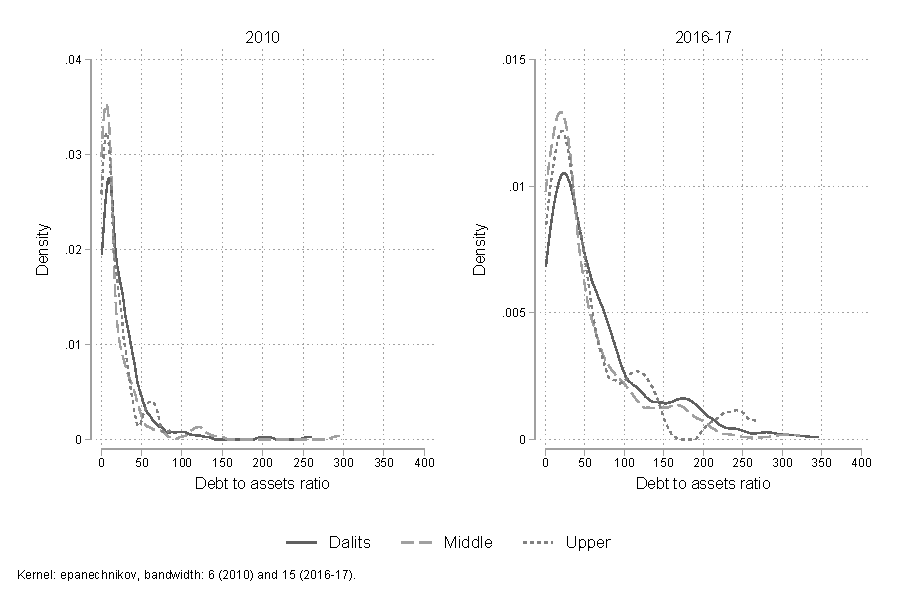
\includegraphics[width=12cm]{DAR_caste.pdf}
\caption{Kernel density of debt to assets ratio by castes}
\sourcefig{RUME (2010) and NEEMSIS (2016-17); author's calculations}
\label{kernel:DARcastes}
\end{figure}

\begin{figure}[h!]
\center
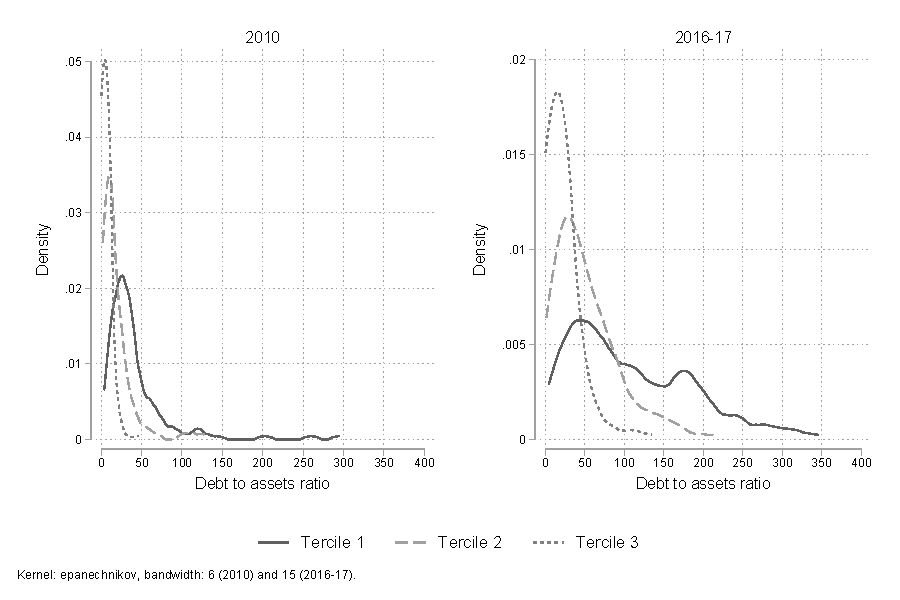
\includegraphics[width=12cm]{DAR_tercile.pdf}
\caption{Kernel density of debt to assets ratio by assets}
\sourcefig{RUME (2010) and NEEMSIS (2016-17); author's calculations}
\label{kernel:DARassets}
\end{figure}



\section{The financial landscape: informal and segmented}
\label{section:finlandscape}

Despite massive efforts in terms of financial inclusion policies over the last two decades \citep{Nair2016, Kar2018}, formal finance, regulated by the state and based on written contracts, accounts for only 29 percent of the amounts borrowed at the household level in terms of volume. 
Formal finance includes ``finance'' (microfinance companies) and banks. 
Finance targets exclusively women. 
Dalits and casual daily labourers are also over-represented (Appendix, Table \ref{appendix:clientelecaste} and \ref{appendix:clienteleocc}). 
Banks are restricted to men, landowners and farmers. 

At the household level, more than two-thirds of the loan volume therefore continues to come from informal or semi-formal sources. 
Among the informal sources, ``well-known persons'' (WKP) --the term locally used-- are the most important sources in terms of number of loans, users and volume (almost a third of loan volumes, and 70 percent of users). 
This category includes a wide range of profiles: a few castes specialising in lending, but above all, a wide range of people for whom lending is not a profession and who have surplus cash to invest, mostly landowners, local entrepreneurs and wage earners. 
The figure of the ``moneylender'', which is often used to describe rural usury, does not really exist, as is also observed in other parts of India \citep{Gregory1997}. 
Next come the relatives, then employers and labour recruiters (``labour'' category). 
The latter are over-represented among Dalits and take the form of wage advances, which are repaid through labour, but at lower rates, and often entail freedom restrictions. 
Pawnbrokers are another fundamental source, especially for women. 
We qualify them as semi-formal because many operate without a license while still lending on the basis of a written contract. 

During the survey period, finance and pawnbroking have grown in importance, both in terms of users and in terms of volume (see Figure \ref{bar:clientele} and Figure \ref{bar:loaned}). 
This increase was at the expense of other sources, notably Self-Help-Groups (SHGs)\footnote{SHGs were India's first microcredit model. SHGs are groups of 15 to 20 people, mainly women, who first circulate money among themselves and are then eligible for external credit, provided by an NGO, a microcredit institution or a bank. In the region studied here, with the advent of for-profit microcredit companies, SHGs have all but disappeared. However, joint liability groups are still the main collateral.}  and debt-labour arrangements. 
However, WKP and relatives remain the predominant form of borrowing.

\begin{figure}[ht]
\center
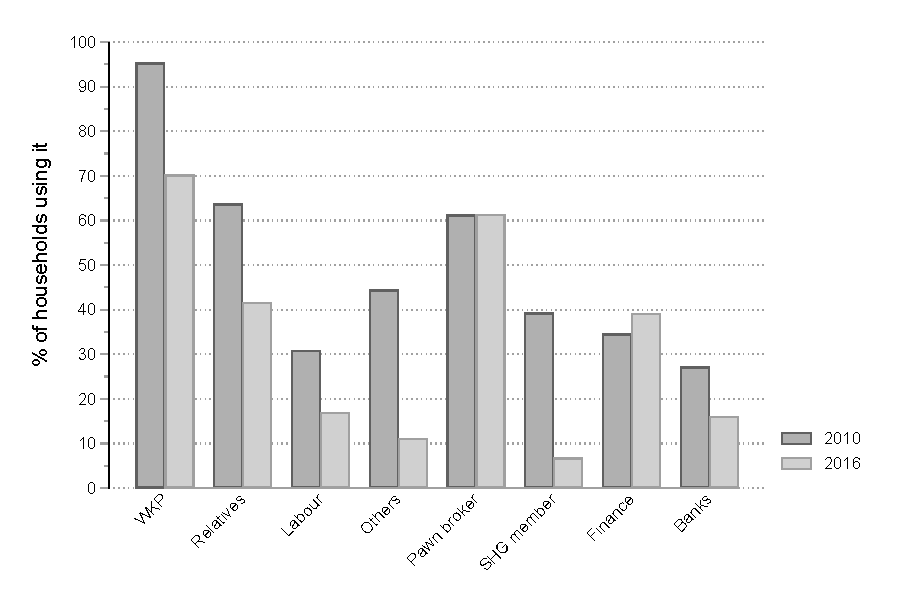
\includegraphics[width=12cm]{totalclientele.pdf}
\caption{Source of borrowing (percent of users)}
\sourcefig{RUME (2010) and NEEMSIS (2016-17); author's calculations}
\label{bar:clientele}
\end{figure}

\begin{figure}[ht]
\center
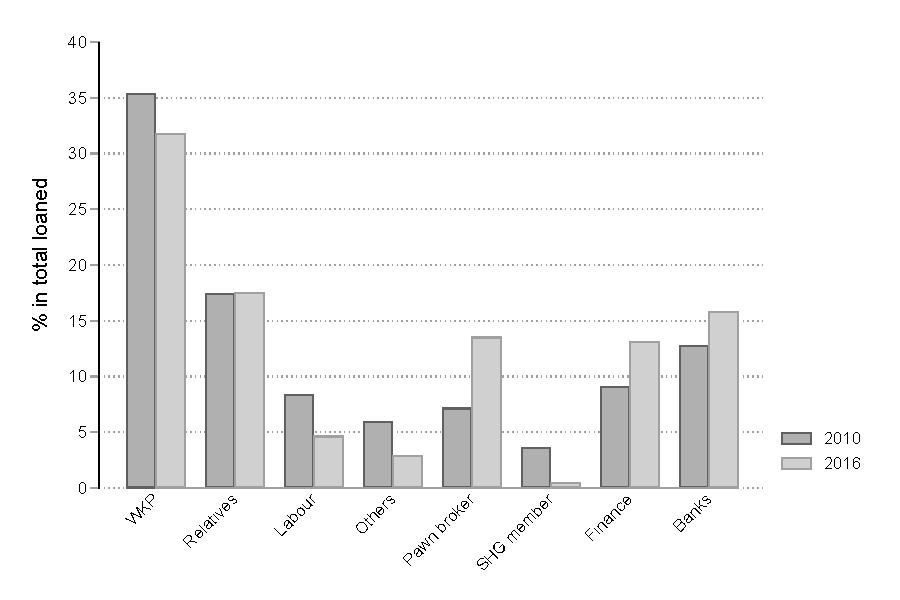
\includegraphics[width=12cm]{totalloaned.pdf}
\caption{Source of borrowing (percent volume)}
\sourcefig{RUME (2010) and NEEMSIS (2016-17); author's calculations}
\label{bar:loaned}
\end{figure}

As observed elsewhere\footnote{See for instance \cite{Morvant2013, Collins2009, Shipton2007, James2015, Saiag2020, Guerin2013}.}, informal sources persist, for several reasons. 
They are very flexible, which is crucial given the irregularity of income. 
For 84 percent of informal loans, the terms are not fixed in advance and borrowers repay when they can. Contrary to what is often claimed in the literature or media, their cost is not, on average, higher than formal sources in the region studied here \citep{Reboul2019}. 
Almost none of them require collateral (79.97 percent require only personal informal agreement). 
Subjective creditworthiness, reputation and trust (the three terms are equivalent in Tamil - \textit{nambikai}) are the key factors in lenders' selection. 

The transformation of sources of borrowing is both shaped by and constitutive of deeper social transformations, including regarding the use and building of trust.
Historically, access to credit, for the landless and small landowners, was mainly based on their labour power, used as collateral and legitimized by caste hierarchies and the possible use of violence\footnote{Historically, Dalits depended on their landlords for access to credit, which was repaid in the form of labour. As elsewhere, these old and agrestic forms of bonded labour have all but disappeared, replaced by neo-bondage, which is limited in time and based on seasonal migration as discussed above \citep{Breman1974}. Jan Breman's pioneering observations are also valid here.}. 
Non-agricultural employment and migration have opened up new opportunities. 
In the village itself, new providers are present. 
In addition to microcredit organizations, many WKPs actually act as informal intermediaries for urban financial lenders. 
Another form of caste segmentation is worth noting, a legacy of a persistent Hindu theology of debt \citep{Kane2012}. 
As the villagers often say, ``you don't borrow from anyone lower than you''. 
Interestingly, however, the Dalits are borrowing more and more from other Dalits (Figure \ref{cont:loans} and \ref{cont:volume}) (and this caste retreat is also observed in other castes)\footnote{We shall note the existence of internal Dalit hierarchies, the term being a political category that in fact includes many \textit{jatis} (castes).}.  

\begin{figure}[h!]
\center
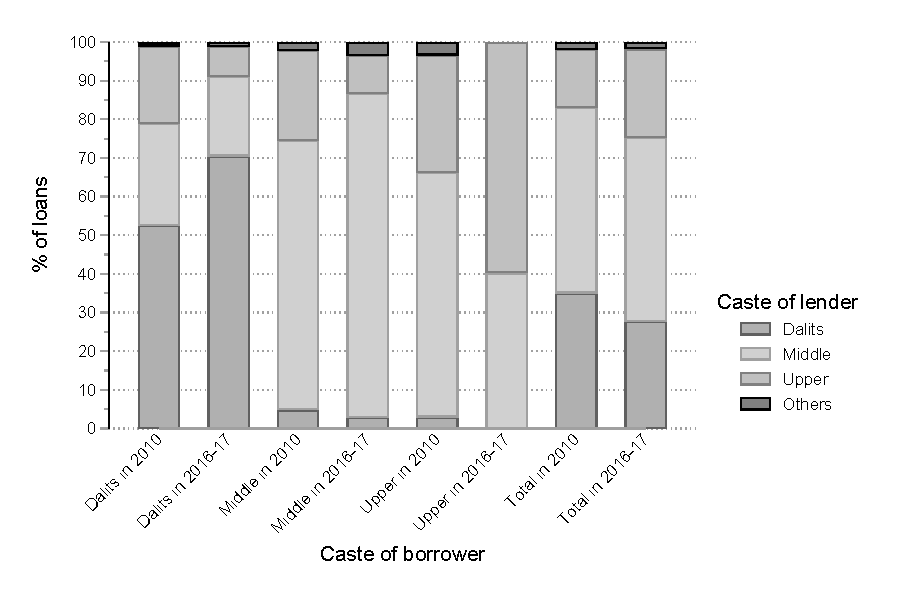
\includegraphics[width=12cm]{contengency_borrower_loan_stata.pdf}
\caption{Debt and caste: who borrows from whom (percent loans)?}
\sourcefig{RUME (2010) and NEEMSIS (2016-17); author's calculations}
\label{cont:loans}
\end{figure}

\begin{figure}[ht!]
\center
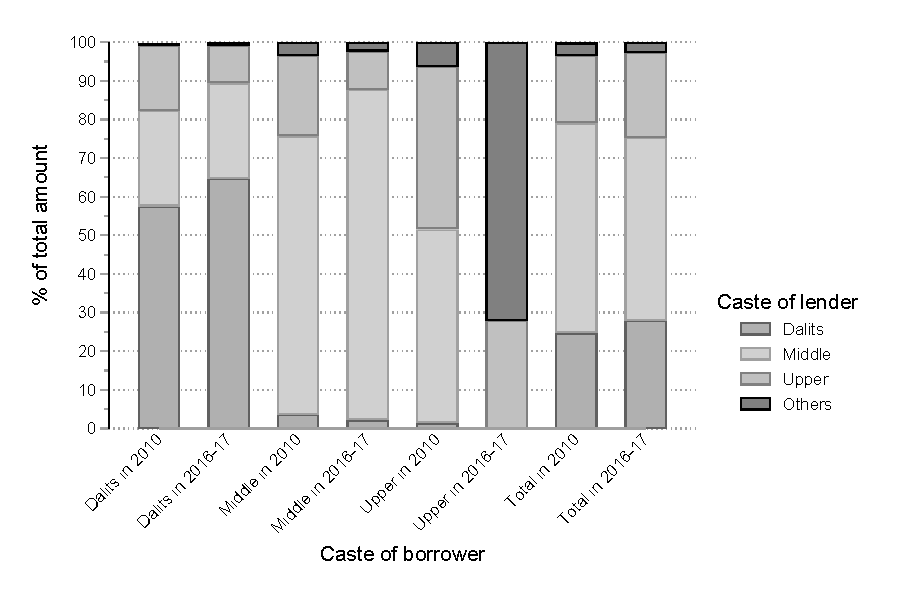
\includegraphics[width=12cm]{contengency_borrower_amount_stata.pdf}
\caption{Debt and caste: who borrows from whom (percent volume)?}
\sourcefig{RUME (2010) and NEEMSIS (2016-17); author's calculations}
\label{cont:volume}
\end{figure}

Trust does not mean blind faith on others, but the ``the negotiation of risk occasioned by the freedom of others'' \citep[p.188]{Hart2000}. 
Broadly speaking, trust depends on the personal and social characteristics of the contracting parties and their respective appreciation, on a process and memory of repeated interactions, and finally on social institutions, broadly defined as the set of rules, norms and conventions that regulate the behaviour of others \citep{Platteau1994}. 
The assessment of incentives and enforcement mechanisms is crucial, and depends on sanctions, the risk of loss of reputation or the risk of loss of reciprocity in case of interdependence. 
For loans among relatives and microcredit loans, which remain based on the principle of group lending, interdependence nurtures trust. 
This does not, of course, exclude tensions and conflicts, whether within kinship or microcredit groups \citep{Kar2018}. 
These are omnipresent. 
But the interdependence is such that relatives and group members remain bound by ties of mutual debt and cannot afford to fail. 

For loans contracted from WKP, several factors come into play.
Even if no collateral is required, the lender takes into account in his or her own assessment material assets --which borrowers can sell if they have difficulty repaying-- and their ability to work. 
Migrants clearly have an advantage and labour recruiters may even be asked to act as guarantors for the first loans. 
As with any lender, the fabric of trust is then based on credit history and repayment behaviour. 
Reputation is public information, available at the village level. 
Reputation encompasses family history, seriousness and ``morality'' of different family members. 
Bad payers are quickly identified and discriminated against by lenders, but also by employers or labour intermediaries. 
They may also affect children’s marriage. 
Reputation is therefore an essential asset in households’ portfolios, which people constantly seek to preserve and cultivate. 
Here too, conflicts are legion. 
Disappearing from the village for a while can be a way of postponing a debt. 
But permanent migration remains exceptional and the attachment to the village is such that payment defaults are rare.

\section{Suspension of repayment}
\label{section:repayment}

When the lockdown was announced, the villagers expressed three major concerns: the loss of jobs, of course; the omnipresent and violent police checks, which exacerbated the climate of anxiety; and the repayment of debts, especially women. 
They discussed first about microcredits, since microcredits are the only ones with rigid and non-negotiable repayment terms. 
Repayments (most often monthly) are often a headache, since cash is constantly in short supply. 
The most organised borrowers regularly save small amounts; the others, in the days before the due date, spend part of their time finding money here and there by soliciting neighbours, friends, husbands and other relatives. 
Soon after the lockdown announcement, however, the Reserve Bank of India (RBI) announced a moratorium on repayments. 
Initially limited to banks, microfinance companies (most of which have non-banking financial company status) had to apply to the RBI to also be eligible for the moratorium. 
However, not all financial companies are complying with the moratorium. 
Some require electronic applications, while many womens are illiterate and most have no access to the internet. 
Other companies give phone calls, requesting women to repay, and our region seems to be no exception\footnote{\url{https://www.thehindu.com/news/cities/Madurai/collector-warns-against-violation-of-rbi-norms-on-loan-moratorium/article31664789.ece/amp/}; \url{https://www.thehindu.com/news/national/tamil-nadu/private-finance-firms-putting-pressure-on-self-help-group-women-says-rajapalayam-mla/article31663098.ece}}.
In the cases we came across, women are well-informed and refuse to let this happen, as the following testimony illustrates, but this requires negotiation and collective organisation. 

\begin{quote}
``The staff is torturing us daily by phone and giving warning that if we fail to repay in the due date, we have to pay interest to interest. 
But I strongly said that we can’t repay right now. 
You can arrest us or do whatever you can. 
How many months have we paid without fail? [...] They think if they ask the payment in an intimidating tone, people will be afraid and will settle the amount. 
I request the [name of the financial company] that I don’t have money to repay. 
I gathered all the members of the group and asked about their situation because I am the head of the group. 
Our members were crying and said that we don’t have income to repay. 
So far we have been paying properly, why are they giving pressure? Then I contacted [name of the financial company] and I told them if you were pressuring us again and again, we will register a complaint against you. 
Then only they stopped contacting us.''
\end{quote}

With regard to informal loans, many creditors try to get their money back, but most of the time without success.
They do not have the means to enforce repayments, and they also have to preserve their reputation. 
``I also borrow elsewhere, how can I shout?'', we often hear. 
While this suspension of repayments may relieve household budgets, it raises the question of how it will affect trust and reputation, one of the most valuable assets that people possess.

\section{Stopping unsecured debt and the loss of trust}
\label{section:trust}

With the lockdown, and the immense uncertainty that goes with it, unsecured debts have stopped. 
While money usually circulates all the time (as does food --a kilo of rice, a glass of oil, a liter of milk), this circulation has stopped, except among very close relatives or very close friends. 
While during the demonetization we observed an extension of networks (and people often compare the two situations), here it is the opposite reaction. 
People have not lost trust in others, but in the future. 
Many mention the ``collapse of trust'' (\textit{nambikai pochu}). 
Uncertainty about the future prevents any trust. 
``People close their doors'' we have been told again and again. 
In the first days, solidarity and sharing was there, but once people have realized that the situation was going to last, they turned in on themselves, as illustrated by the following testimonies:
\begin{quote} 
``Usually neighbors, sister in law, god will come… now no one is coming.''
\end{quote}
\begin{quote}
``If there is any crisis, always someone is there to support, now all doors are closed.'' 
\end{quote}
\begin{quote}
``There is no food, there is no cash, I have to find a way to protect myself; even the government says, close the doors, stay inside.'' 
\end{quote}
\begin{quote}
``No one is ready to give. 
All say ‘we don’t have enough money’. 
Moreover we don’t ask money from neighbors and relations. 
Our only believe is daily coolie work.''
\end{quote}
\begin{quote}
``Even \textit{kaimathu} [help from hand to hand], that's impossible. 
Everyone closes the door and does not want to talk to us. 
They fear that people won't return the money. 
People plan that it may last for one year. 
My village is empty. 
No-one wants to see us.''
\end{quote}
\begin{quote}
``Nobody wants to help […].
Everybody is in some sort of trauma to say they have cash. 
They even hide to their close relatives.'' 
\end{quote}

A milk trader whom we know well, who did whatever he could at the time of demonetization to support his network of producers, told us: ``don’t ask anything!''.
We shall also give the example of this labour recruiter, Dalit, whom we have known for fifteen years. 
We have seen him gradually build up his network of workers and creditors, which he needs to provide wage advances. 
Over the years, he has built up an excellent reputation by regularly protecting his workers (loans or gifts in case of illness, unforeseen events, etc.). 
He can count on four trusted creditors (well-known persons) with whom he has gradually built relationships. 
Today he can neither repay his creditors nor help his workers. 
Many of them are now waiting for him in front of his house, hoping for some kind of help. 
He avoids being him. 
He turns his phone off and on for only a few minutes a day. 
He calls us in desperation. 
He goes so far as to talk about suicide. 
His haunting, he tells us, is to lose his \textit{nambikai} (reputation).

It is known that in many informal economies, the pressure for redistribution limits the scope for accumulation \citep{Platteau2015, Nguyen2017}. 
Here, it is experienced by people as a threat to their survival. 
Thus these two co-wives, who remain hidden at home because they are indebted to several women in the neighbourhood. 
Their son tells us that they no longer dare to go out because they would feel obliged to give what little they have. 
At the same time they feel terribly guilty.

Fear of the future and the loss of the usual networks of protection leads to considerable anxiety --people keep asking when the lockdown will end, and more importantly, when economic activity will resume. 
Returning to old dependencies, from which many Dalits had tried to extricate themselves, is an alternative.
This is the case of this Dalit woman:

\begin{quote}
``A woman, I know her for the last thirty years, we watch TV together, here or vice versa. 
I often acted as a guarantor for her; but she refused [to help]. 
She thinks I may not be able to return the 5 kg rice, as my family is big. 
Corona is closing my door. 
She is like my sister. 
Now my only choice is I am going to a Mudaliyar [upper caste]. 
My father in law was attached labourer there. 
He died but his son is still there. 
I will have to explain: my father in law was attached labour there, I have to build a new relation.'' 
\end{quote}

Together with other women, she manages to convince the Mudaliyar to plant cucumber and black gram and hire them. 
It's embarrassing to go begging, she says, since her family was out of this dependency, but she has no choice, ``he's the only one who feeds us''. 
However, reviving old forms of protection is only possible in irrigated villages. 
In the dry villages, workers are desperately waiting for transport to start up again. 
We have to go and move, whatever the destination and the activity, they say.  

\section{The emergence of new forms of secured debt: a risk of massive depletion?}
\label{section:newforms}

We have seen above the widespread use of pawnbrokers. 
Because of the crucial role of gold as savings (both precautionary and long-term savings), households buy gold whenever they can. 
The median amount owned increased significantly over the period but only for non-Dalit. 
For Dalits, it decreased by 20 percent (from 40g to 32g). 
For all castes, about two thirds of the gold is pawned at the time of the survey. 

With the lockdown, pawnbrokers were forced by regulation to close for almost two months. 
A few managed to operate from home. 
At the end of May, the others have started to reopen, but their activity is limited, probably due to scarce liquidities. 
At the same time, old practices are re-emerging: pawnbroking within the village, between landowners' wives (now, mainly middle castes) and those who are severely lacking in liquidity (mostly non-farm daily labourers). 
This practice was widespread when the landless or smallholders depended mainly on agriculture, and access to credit was limited. 
Due to lack of income, and lack of visibility on their future income, many households have lost their creditworthiness. 
Conversely, potential lenders face themselves many uncertainties and don’t want to take risk.  
With the loss of trust, pledging assets has become the only way to secure financial transactions. 
Pawning a piece of jewellery just to eat is a heartbreaker, especially for non-Dalits. 
Historically, pawnbroking was reserved for agricultural investment: pledging gold to eat is a habit of ``poor'', often considered as a Dalit stigma. 
The deal is also unusual: instead of obtaining a lump sum (usually three-quarters or two-thirds of the jewel’s value), small sums are disbursed regularly. 
Lenders cannot afford more, and borrowers only ask for the minimum, to avoid being approached in their turn by their close circle. 
Thus this lady who pledges a piece of jewellery worth INR 30,000, borrows INR 800, then comes back a few days later to borrow INR 500. 
Another deposits a piece of jewelry worth INR 15,000, borrows INR 500, and a week later borrows INR 1,000. 
We can assume they will come regularly according to their needs as long as the job shortage lasts. 
For households who do not find employment quickly, which is likely to be the case in the non-farm sector, one may expect a massive loss of their gold assets. 

Land raise similar concerns. 
Almost half households (46 percent) have lost land over the period. 
The share of landowners fell from 42 percent to 21 percent, and each caste experienced a similar decline (see Table \ref{Global}). 
Qualitative surveys indicate that indebtedness is often an explanatory factor. 
Land is very rarely mortgaged, but the people have no other choice than selling it when they can no longer pay their creditors. 
Here too, new forms of secured loans are being developed, especially for bonded labourers. 
As mentioned above, part of our sample make a living thanks to seasonal migration and wage advances. 
With the lockdown, most have returned. 
Not only they have lost their source of livelihood but they are heavily indebted, with amounts ranging from 70,000 to INR 100,000. 
Employers are very unlikely to write off this debt. 
Whether it is the brick producers or the sugar mills, they themselves are in great trouble. What is more, among the brick kiln owners, some have even started to threaten their workers by demanding title deeds, something that has never happened before: until now the only collateral was labour. 
Given the uncertainty about the future, labour is no longer a collateral. 
Far beyond our case study, activists and researchers are concerned that the lockdown could lead to the emergence of new forms of slavery (\citealp{Nagaraj2020}; \citealp[p.14]{Sahas2020}).   

\section*{Discussion and conclusion}
\label{section:conclusion}
In different regions of the world, the pandemic --and the lockdown (whose effects are currently greater than the pandemic itself, in some contexts such as India)-- have exposed pre-existing fragilities: insufficient health systems, excessive concentration of production chains, devaluation of essential workers, suddenly becoming visible, etc. 
As our case study shows, the fragility of growth based on private debt is also exposed. 
With the lockdown, not only have workers lost their sources of income, albeit unevenly, but they are unable to repay their debts. 
In the region studied, debt has exploded over the past decade. 
While debt was already a source of financial fragility and decapitalization for part of the population, there is concern that the lockdown could accentuate this trend. 
The only credits accessible during the lockdown are secured credits, based on gold or land.
Our case study is limited to a specific region and has no claim to generalization. 
However, the sharp increase in private debt observed in many developing countries before the pandemic, and which was already a source of concern \citep{WorldBank2020, UNCTAD2019, UN2020}, really deserves a particular attention.

In India, farmers’ debt and its consequences in terms of suicide has been a known and debated fact for several decades \citep{Mohanty2005}. 
While rural incomes are now mostly non-farm (and this is true for India in general), the extent of indebtedness in rural areas, beyond farmers, has not yet been measured. 
Until now, internal migration and the regular injection of liquidity (through microcredit, but also and above all through informal urban financiers) explained the sustainability of this debt system. 
Migration income and new debts repay old debts. 
Debt is chronic and its repayment takes a large part of the income, acting in fact as a rent-seeking system for lenders. 
Moreover, the slightest contingency is a major source of fragility and impoverishment, when the sale of assets is the only way to repay the debt. 
When the crisis is systemic, as is the case here, we can fear a massive collapse. 
Beyond material assets, it is also personal relationships, trust and reputation that are threatened. 
In a predominantly informal economy, these social assets are extremely valuable \citep{Hart2000, Platteau1994}.

The gender of our findings are also worth mentioning. 
As those responsible for meal preparation, managing family budgets and increasingly, household debt \citep{Guerin2019}, women are on the front line of the lockdown. 
Jewelry is the few things they own, as most are still deprived of land ownership. 
When it comes to eating less, they are certainly the first to sacrifice themselves. 
When the moratorium on formal debts is lifted, they will still be in the front line since they are the main clients of microcredit organizations. 
A specific analysis would be necessary, and a comparison with the gendered effects of famines would certainly be useful \citep{Cliggett2005, Rangasami1986}. 

The debt of the poor is often debated: is it a survival debt simply to make ends meet or to cope with life's accidents, or does it reflect expensive and ostentatious behaviour? 
As early as colonial times, British officials and Christian missions were concerned about the massive indebtedness of peasants, which was described as a ``congenital propensity for extravagance'' \citep[p.167]{Pouchepadass1980}. 
Debt is above all the result of unequal societies \citep{UN2020}, which on the one hand do not offer the poorest their basic needs, forcing them to go into debt to make a living, and which on the other hand give rise to social needs and envy, that result from a search for dignity \citep{Servet2013}. 
This need for dignity is less present in societies of status, where there is usually a consensus on the acceptance of hierarchies and rank. 
In the region studied here, Dalits, as we have mentioned, have fought tirelessly to extricate themselves from a caste status society. 
Debt, together with internal migration, has been precisely a vehicle for this search of (relative) independence. 
Credit, the other side of debt, is a promise about the future: by allowing borrowers to project themselves into the future and to hope, debt has made it possible to create or to fulfil aspirations, something of which the subordinates are often the most deprived \citep{Appadurai2004}. 
But to be eligible for credit, people have to build creditworthiness. 
Honouring commitments is no longer based on status or fear of violence. 
Nor is it based on contract, which is of little value in a context like India \citep{Harriss-White2003} as in many other developing countries \citep{Platteau1994}. 
The trust needed to access credit is based on experience and repeated interactions \citep{Hilger2020} on various forms of incentives such as the threat of jeopardy of reputation, and on reciprocity and interdependence (with relatives and peers). 
Caste-based hierarchical bonds have become greatly distended. 
Kinship ties, as we have seen, remain a major asset, but they are articulated with other relationships built and cultivated over time. 
Yet, access to off-farm income sources, although uncertain and unpredictable, was a precondition of trust. 
With the drying up of income sources, trust has disappeared, at least temporarily, and reputation is under serious threat. 
While debt is now the only way to survive, secured credit, based on gold or land, is the only option.
What will be left of these assets, both material and social? 
Only time will tell.

What is certain, however, is that for the poorest, current forms of protection remain very fragile. 
This is true of the protection provided by the State, whose redistribution exists but remains insufficient, erratic and unequal. 
This is true of kin protection, which can come into play in times of growth but is necessarily limited in times of systemic crisis. 
This is true of the relations recently created outside the kin circle, both within the caste and outside it. 
These are based on a trust built up over time, but which the systemic crisis seems to have destroyed.
The lockdown follows various measures taken by the BJP-led government of Narendra Modi done since 2014 (demonetization, Goods and Services Tax reform) which strongly suggests that the aim is to “destroy” the informal economy \citep{Harriss-White2020}. 
One can imagine that the big players in this informal economy, organized around mafia-clans, will know how to adapt and have already been able to do so. 
For the others, the vast majority and those discussed here, this destruction seems to be well under way.

%\bibliographystyle{elsarticle-harv} % (For authoryear Elsevier citations)

% The bibliography file
\bibliography{Biblio}

\newpage
\appendix
\section{Appendix}

% Table generated by Excel2LaTeX from sheet 'Table 3'
\begin{table}[htbp]
  \center
  \caption{Purpose of loans}
       \resizebox{\columnwidth}{!}{%          
    \begin{tabular}{lcccccccccccccc}
    \toprule
      & \multicolumn{2}{c}{Number of loans} &   & \multicolumn{2}{c}{\% of loans} &   & \multicolumn{2}{c}{\% of HH using it} &   & \multicolumn{2}{c}{Mean (1,000 INR)} &   & \multicolumn{2}{c}{\% in the total loand} \\
\cmidrule{2-3}\cmidrule{5-6}\cmidrule{8-9}\cmidrule{11-12}\cmidrule{14-15}      & 2010 & 2016 &   & 2010 & 2016 &   & 2010 & 2016 &   & 2010 & 2016 &   & 2010 & 2016 \\
    \midrule
    Economic investment &   &   &   &   &   &   &   &   &   &   &   &   &   &  \\
    \hspace*{0.2cm} \textit{Agriculture} & 380 & 181 &   & 19.42 & 8.91 &   & 47.90 & 18.48 &   & 25.29 & 62.73 &   & 23.08 & 14.89 \\
    \hspace*{0.2cm} \textit{Investment} & 98 & 105 &   & 5.01 & 5.17 &   & 14.81 & 13.96 &   & 40.99 & 83.79 &   & 9.65 & 11.54 \\
    Current expenses &   &   &   &   &   &   &   &   &   &   &   &   &   &  \\
    \hspace*{0.2cm} \textit{Family} & 528 & 542 &   & 26.98 & 26.69 &   & 73.33 & 57.49 &   & 10.67 & 18.43 &   & 13.53 & 13.10 \\
    \hspace*{0.2cm} \textit{Repay previous loan} & 87 & 95 &   & 4.45 & 4.68 &   & 18.52 & 16.43 &   & 18.80 & 27.67 &   & 3.93 & 3.45 \\
    \hspace*{0.2cm} \textit{Relatives} & 102 & 13 &   & 5.21 & 0.64 &   & 23.70 & 2.05 &   & 10.73 & 11.71 &   & 2.63 & 0.20 \\
    Human capital &   &   &   &   &   &   &   &   &   &   &   &   &   &  \\
    \hspace*{0.2cm} \textit{Health} & 202 & 157 &   & 10.32 & 7.73 &   & 35.06 & 20.12 &   & 27.14 & 26.74 &   & 13.17 & 5.51 \\
    \hspace*{0.2cm} \textit{Education} & 149 & 167 &   & 7.61 & 8.22 &   & 26.67 & 21.77 &   & 20.19 & 31.60 &   & 7.22 & 6.92 \\
    Social &   &   &   &   &   &   &   &   &   &   &   &   &   &  \\
    \hspace*{0.2cm} \textit{Ceremonies} & 69 & 127 &   & 3.53 & 6.25 &   & 15.56 & 20.53 &   & 13.01 & 21.24 &   & 2.16 & 3.54 \\
    \hspace*{0.2cm} \textit{Marriage} & 137 & 317 &   & 7.00 & 15.61 &   & 22.72 & 26.69 &   & 33.20 & 53.73 &   & 10.92 & 22.34 \\
    \hspace*{0.2cm} \textit{Death} & 17 & 26 &   & 0.87 & 1.28 &   & 3.70 & 4.52 &   & 14.41 & 14.62 &   & 0.59 & 0.50 \\
    Housing &   &   &   &   &   &   &   &   &   &   &   &   &   &  \\
    \hspace*{0.2cm} \textit{House exp} & 188 & 271 &   & 9.61 & 13.34 &   & 29.38 & 28.13 &   & 29.08 & 39.64 &   & 13.13 & 14.09 \\
    Other &   &   &   &   &   &   &   &   &   &   &   &   &   &  \\
    \hspace*{0.2cm} \textit{No reason} & 0 & 3 &   & 0.00 & 0.15 &   & 0.00 & 0.62 &   & 0.00 & 51.83 &   & 0.00 & 0.20 \\
    \hspace*{0.2cm} \textit{Other} & 0 & 27 &   & 0.00 & 1.33 &   & 0.00 & 4.31 &   & 0.00 & 104.78 &   & 0.00 & 3.71 \\
      &   &   &   &   &   &   &   &   &   &   &   &   &   &  \\
    Total & 1957 & 2031 &   & 100.00 & 100.00 &   & 405 HH & 487 HH &   & 21.28 & 37.54 &   & 100.00 & 100.00 \\
    \bottomrule
    \end{tabular}%
	}
  \label{appendix:purpose}%
	\sourcetab{RUME (2010) and NEEMSIS (2016-17); author's calculations}
\end{table}%

% Table generated by Excel2LaTeX from sheet 'Sheet3'
\begin{table}[htbp]
  \center
  \caption{Loan sources by caste and ownership}
    \begin{tabular}{lrrrrrrr}
    \toprule
          & \multicolumn{1}{c}{Total} &       & \multicolumn{1}{c}{Dalits} & \multicolumn{1}{c}{Non dalits} &       & \multicolumn{1}{c}{Land owner} & \multicolumn{1}{c}{Not land owner} \\
    \midrule
    Number of household & n=487 &       & n=232 & n=255 &       & n=153 & n=334 \\
    All sources & 100.00 &       & 100.00 & 100.00 &       & 100.00 & 100.00 \\
    Informal &       &       &       &       &       &       &  \\
    \hspace*{0.2cm} \textit{WKP} & 70.23 &       & 70.26 & 70.20 &       & 67.97 & 71.26 \\
    \hspace*{0.2cm} \textit{Relatives} & 41.68 &       & 41.81 & 41.57 &       & 47.06 & 39.22 \\
    \hspace*{0.2cm} \textit{Labour} & 17.04 &       & 21.12 & 13.33 &       & 3.92  & 23.05 \\
    \hspace*{0.2cm} \textit{Others} & 11.09 &       & 11.21 & 10.98 &       & 11.76 & 10.78 \\
    Semi formal &       &       &       &       &       &       &  \\
    \hspace*{0.2cm} \textit{Pawn broker} & 61.40 &       & 58.62 & 63.92 &       & 64.71 & 59.88 \\
    \hspace*{0.2cm} \textit{SHG member} & 6.78  &       & 6.90  & 6.67  &       & 5.88  & 7.19 \\
    Formal &       &       &       &       &       &       &  \\
    \hspace*{0.2cm} \textit{Finance} & 39.22 &       & 44.40 & 34.51 &       & 40.52 & 38.62 \\
    \hspace*{0.2cm} \textit{Banks} & 16.02 &       & 9.05  & 22.35 &       & 28.10 & 10.48 \\
    \bottomrule
    \end{tabular}%
  \label{appendix:clientelecaste}%
  	\sourcetab{NEEMSIS (2016-17); author's calculations}
\end{table}%

% Table generated by Excel2LaTeX from sheet 'Sheet3'
\begin{table}[htbp]
  \center
  \caption{Loan sources per occupation (main occupation of the household head)}
       \resizebox{\columnwidth}{!}{%          
    \begin{tabular}{lrrrrrrrrr}
    \toprule
          & \multicolumn{1}{c}{Total} &       & \multicolumn{1}{c}{Agri. SE} & \multicolumn{1}{c}{Agri. Casual} & \multicolumn{1}{c}{Casual} & \multicolumn{1}{c}{Regular non quali} & \multicolumn{1}{c}{Regular quali} & \multicolumn{1}{c}{SE} & \multicolumn{1}{c}{NREGA} \\
    \midrule
    Number of household & n=487 &       & n=103 & n=108 & n=75  & n=81  & n=10  & n=87  & n=23 \\
    All sources & 100.00 &       & 100.00 & 100.00 & 100.00 & 100.00 & 100.00 & 100.00 & 100.00 \\
    Informal &       &       &       &       &       &       &       &       &  \\
    \hspace*{0.2cm} \textit{WKP} & 70.23 &       & 65.96 & 75.00 & 76.47 & 64.86 & 55.56 & 67.09 & 76.19 \\
    \hspace*{0.2cm} \textit{Relatives} & 41.68 &       & 54.26 & 50.00 & 41.18 & 20.27 & 66.67 & 39.24 & 42.86 \\
    \hspace*{0.2cm} \textit{Labour} & 17.04 &       & 3.19  & 8.00  & 23.53 & 56.76 & 0.00  & 7.59  & 9.52 \\
    \hspace*{0.2cm} \textit{Others} & 11.09 &       & 12.77 & 11.00 & 10.29 & 9.46  & 33.33 & 10.13 & 4.76 \\
    Semi formal &       &       &       &       &       &       &       &       &  \\
    \hspace*{0.2cm} \textit{Pawn broker} & 61.40 &       & 63.83 & 53.00 & 63.24 & 63.51 & 77.78 & 62.03 & 85.71 \\
    \hspace*{0.2cm} \textit{SHG member} & 6.78  &       & 3.19  & 7.00  & 8.82  & 8.11  & 22.22 & 5.06  & 9.52 \\
    Formal &       &       &       &       &       &       &       &       &  \\
    \hspace*{0.2cm} \textit{Finance} & 39.22 &       & 27.66 & 39.00 & 45.59 & 25.68 & 66.67 & 56.96 & 33.33 \\
    \hspace*{0.2cm} \textit{Banks} & 16.02 &       & 36.17 & 12.00 & 4.41  & 10.81 & 22.22 & 10.13 & 28.57 \\
    \bottomrule
    \end{tabular}%
	}
  \label{appendix:clienteleocc}%
  	\sourcetab{NEEMSIS (2016-17); author's calculations}
\end{table}%




\end{document}